\documentclass[a4paper,14pt]{article} 
\usepackage{lscape}
%%% Страница
\usepackage{extsizes} % Возможность сделать 14-й шрифт
\usepackage{geometry} % Простой способ задавать поля
        \geometry{top=25mm}
        \geometry{bottom=30mm}
        \geometry{left=30mm}
        \geometry{right=20mm}
 %

\usepackage[T1,T2A]{fontenc}
\usepackage[utf8]{inputenc}
\usepackage[english,russian]{babel}
\usepackage{amssymb,amsmath}
\usepackage{float}
\usepackage[unicode, pdftex]{hyperref}
\usepackage[europeanresistors,americaninductors]{circuitikz}
\usetikzlibrary{calc}
\usepackage[T1,T2A]{fontenc}
\usepackage[utf8]{inputenc}

\usepackage{amssymb,amsmath}
\usepackage{float}
\usepackage[unicode, pdftex]{hyperref}
\usepackage{booktabs}
\usepackage{multirow}

\usepackage{tikz}
\usepackage{rotating}
%\usepackage[landscape]{geometry}
\usepackage{graphicx}
\graphicspath{{pictures/}}
\DeclareGraphicsExtensions{.pdf,.png,.jpg}
\usepackage{pgfplots}
\usepackage{wrapfig}
\usepackage{rotating}
\usepackage{lipsum}
\usepackage{nccmath}
\usepackage{caption}
\usepackage{siunitx}
%\usepackage[american,cuteinductors,smartlabels]{circuitikz}
%\usepackage[backend=biber]{biblatex}

\usepackage[]{hyperref}
\ctikzset{bipoles/thickness=1}
\ctikzset{bipoles/length=0.8cm}
\ctikzset{bipoles/diode/height=.375}
\ctikzset{bipoles/diode/width=.3}
\ctikzset{tripoles/thyristor/height=.8}
%\ctikzset{tripoles/thyristor/width=1}
\ctikzset{tripoles/thyristor/width=0.8}
\ctikzset{bipoles/vsourceam/height/.initial=.7}
\ctikzset{bipoles/vsourceam/width/.initial=.7}
\tikzstyle{every node}=[font=\small]
\tikzstyle{every path}=[line width=0.8pt,line cap=round,line join=round]

\ctikzset{resistor = european}
\ctikzset{inductor = american}
\ctikzset{tripoles/thyristor/height=0.55}
\ctikzset{tripoles/thyristor/height 2=0.4}
%\ctikzset{tripoles/thyristor/width=0.35} 
\ctikzset{tripoles/thyristor/diode width left=0.35}
\ctikzset{tripoles/thyristor/diode width right=0.35}

\ctikzset{bipoles/cuteindictor/coils/.initial=3}
\ctikzset{bipoles/americanindictor/coils/.initial=3}
\ctikzset{bipoles/cuteindictor/coils/.initial=3}
\ctikzset{bipoles/americanindictor/coils/.initial=3}
\hypersetup{
colorlinks=false,
}
\usepackage{textcomp}

\begin{document}
%METHODICAL INSTRUCTIONS FOR PERFORMING LABORATORY WORKS

\section{Study of a step-down pulse-width DC-DC converter}

\subsection{Objective}

The study of electromagnetic processes, external, regulatory and energy characteristics of a step-down pulse-width converter at an active-inductive load shunted by a diode.

\subsection{Lab Description}

In this laboratory work, we use: "Bench Power Module"/Модуль питания стенда/ (single-phase), 
"DC-DC Converters"/Преобразователи постоянного напряжения/, "Power Meter"/Измеритель мощности/, "Load"/Нагрузка/ (single-phase), and two-channel oscilloscope modules.

The front panel of the module "DC-DC Converters" is shown in Fig. one.
The transformer circuit UZ1 is presented as a serial (voltage decreasing) key, and UZ2 as a parallel (increasing) key.


%DC CONVERTERS
\begin{figure}[!ht]
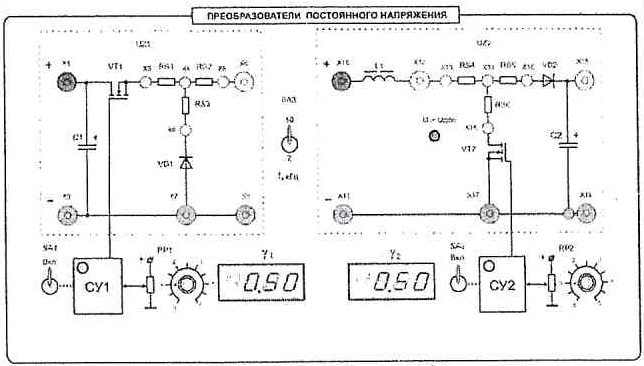
\includegraphics[scale=2]{img_50}
	\caption{The front panel of the module "DC-DC Converters".}
\end{figure}

The serial key is switched on by the toggle switch SA1, and the LED of the SU1/СУ1/ unit lights up.
The fill factor (duty cycle) of the key is regulated by the RP1 potentiometer and is displayed on the adjacent 4-digit indicator.
Similarly, $SA2$ and $RP2$ control the operation of the parallel key.
When the permissible voltage is exceeded on the key, the led "$U>U_\textcyrillic{доп.}$" lights up.
The frequency of switching the keys is determined by the position of the toggle switch SA3.
All shunts $RS1$ - $RS6$ with a resistance of 1 Ohm and are designed to take current waveforms.

\subsection{The task}

\begin{enumerate}
\item Assemble the circuit in accordance with fig. 1.1.

\item Take the waveforms of currents and voltages on the circuit elements for the given parameters.

\item Remove the adjusting $U_{Load}=F(\gamma)$ and energy $P_d=F(\gamma)$, $P_{Load}=F(\gamma)$, $\eta = F(\gamma)$,  $q_i = F(\gamma)$ characteristics of the converter with a constant value of the load resistance $R_{Load}$ and given $U_d$ and $f_{carrier}$.

\item Observe the external $U_{Load} = F(I_{Load})$ and energy $P_d=F(I_{Load})$, $P_{Load}=F(I_{Load})$, 
$\eta = F(I_{Load})$, $q_i=F(I_{Load})$ characteristics at a constant duty cycle $\gamma$ for given $U_d$ and 
$f_{carrier}$.

\item To study the influence of the carrier frequency $f_{carrier}$ on the ripple coefficient $q_i$ of 
	the load current $i_{Load}$.
\end{enumerate}

\subsection{Initial data}

The base point (mode) for which the waveforms are taken and through which the recorded characteristics pass:
\begin{description}
	\item mode -- continuous;

	\item carrier frequency $f_{carrier}=2 kHz$;

	\item duty cycle $\gamma=0.7$;

	\item power supply voltage $U_d=25 V$;

	\item load current $I_{Load} =0.7 A$.
\end{description}
The base point can be changed as instructed by the teacher.

\subsection{Guidelines}

\begin{enumerate}
\item Assemble the circuit for the study of the DC-DC converter in accordance with Fig. 1.1.
Additional external connections are indicated by dashed lines.

Set the preset carrier frequency $f_{carrier}$ with the $SA3$ toggle switch. Set potentiometer knobs $RP1$, $RP2$ to position "0".

Fig. 1.1. Schematic diagram for the study of a step-down DC-DC converter.

		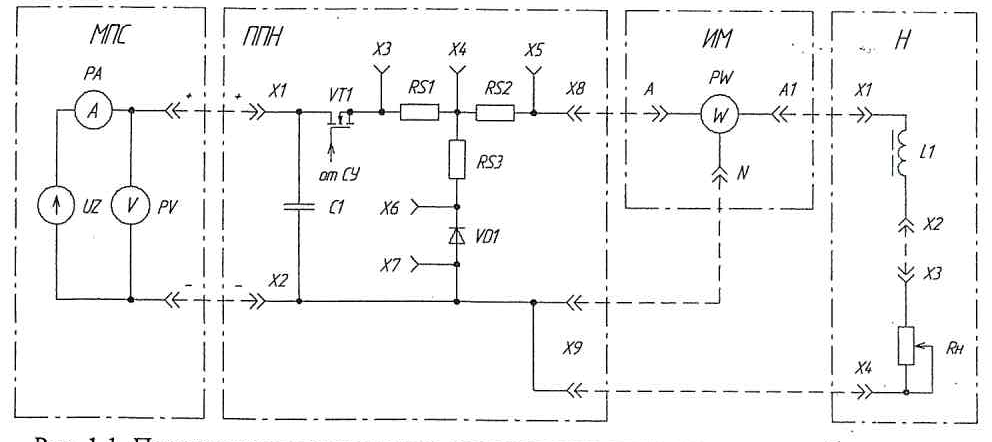
\includegraphics[scale=1.8]{img_51}

Set the handle of the load current regulator $RP$ in the "Load" module (Н) to the "0" position 
	corresponding to the minimum load current (maximum load resistance $R_{Load}$).

Turn on the automatic machine $QF1$ “Stand Power Module” (SPM).

Switch on the "Grid"/"Сеть"/ toggle switch of the “Power Meter” module.
To transfer the “Power Meter” module to the mode of measuring constant currents and voltages, 
	simultaneously press the "$P/Q/S$" and "$f/\cos\varphi/\varphi$" buttons.
Keep the buttons pressed until "DC"/"Постоянный ток"/ appears on the display.
Set measurement limits: toggle switch "U" 30 V, toggle switch "I" 2A.

Toggle switch SA1 to turn on the power of the control system of the "DC/DC Converter" module.
Turn on the power source switch $SA1$ in the SPM module.
Use potentiometer $RP1$ to set the target voltage of the power supply.

\item Take the waveforms of currents and voltages on the circuit elements for the given parameters.

a) take the waveforms of the voltage on the transistor switch $u_{VT}$ and the current through 
		the transistor $i_{VT}$.
To do this, check the desired value of the supply voltage $U_d$ and set the desired value of the duty cycle $\gamma$ with the handle of potentiometer $RP1$ (basic mode).
		Using the current regulator knob $RP$ using the Power meter, set the desired value of the load current $I_{Load}$.
Connect the channel $CH1$ of the oscilloscope to the shunt $RS1$ ("input" - socket $ХЗ$, the case of the oscilloscope $\bot$ -- socket $X4$), and the input of the channel $CH2$ -- to socket $X1$ (voltage on the transistor key).

		{\bf Attention: hereinafter, before taking the oscillograms, check the position of the zero line by moving the switch mode of the input inputs of the amplifiers “AC-GND-DC” to the position “GND”.
		This line is first plotted on the waveform.}

Draw from the oscilloscope screen the waveform.
Define scales by voltage, current and time;

		6) take the waveforms of the voltage on the diode $u_D$ and the current through the diode $i_D$ at the same given values $U_d$, $\gamma$ and $I_{Load}$.
To do this, connect the oscilloscope channel $CH1$ to the $RS3$ shunt ("input" is socket $X6$, 
the oscilloscope case $\bot$ is socket $X4$), and the channel input $CH2$ is connected to socket $X7$. 
	Draw the oscillogram from the oscilloscope screen, preserving the scale;

		c) take the waveforms of the voltage at the load $u_{Load}$ and the load current $i_{Load}$ at the same given values $U_d$, $\gamma$ and $I_{Load}$.
To do this, connect the oscilloscope channel $CH1$ to the $RS2$ shunt ("input" - socket $X4$, 
the oscilloscope case $\bot$ -- socket $X5$), and the channel input $CH2$ -- to socket $X7$ (load voltage).
To obtain a positive voltage deviation $u_{Load}$, press the $CH2$ $INV$ button on the oscilloscope.
Draw waveforms from the oscilloscope screen, keeping the scale.
Using the $i_{Load}$ waveform, determine in what mode the circuit operates (continuous or intermittent current in the load).

\item Observe the adjusting $U_{Load} = F(\gamma)$ and energy $P_d = F(\gamma)$, $P_{Load} = F(\gamma)$, 
	$\eta = F(\gamma)$, $q_i = F (gamma)$ characteristics of the converter at a constant value of
load resistance $R_{Load}$ and given $U_d$ and $f_{carrier}$.
Set basic mode.
		Determine the resistance $R_{Load}$ by the formula

$$
		R_{Load} = U_{Load}/I_{Load}
$$


When taking off the characteristics, do not touch the $RP$ knob in the "Load" module.
By changing the $\gamma$ with the handle of the potentiometer $RP1$ in the range from zero 
to the maximum possible value, record the readings of the instruments $U_d$, $I_d$, $U_{Load}$, $I_{Load}$,
$P_{Load}$ and also use an oscilloscope to measure the amplitude of the ripple of the load current 
$\Delta I_{Load}$.
To do this, switch the oscilloscope channel $CH1$ to the open input "AC" (variable component of the input signal).
Measure the double amplitude of the ripple of the load current $\Delta I_{Load}$.
Measure $\Delta I_{Load}$ only in the area of continuous current.
The reading put in table 1.1.
Mark the transition point from continuous to intermittent (boundary current).

\begin{tabular}{l|p{10pt}|p{10pt}|p{10pt}|p{10pt}|p{10pt}|p{10pt}p{80pt}}
	$\gamma$ & &&&&&& notes\\
	\cmidrule{1-8}
	$U_d$, V &&&&&&&\multirow{9}{*}{\begin{minipage}{0.3\textwidth}$R_L=$,\\$f_{carrier}=$\end{minipage}}\\
	\cmidrule{1-7}
	$I_d$, A &&&&&&\\
	\cmidrule{1-7}
$U_L$, V &&&&&&\\
	\cmidrule{1-7}
	$I_L$, A &&&&&&\\
	\cmidrule{1-7}
	${\scriptstyle \Delta}I_L,A$&&&&&&\\
	\cmidrule{1-7}
$q_i$ &&&&&&\\
	\cmidrule{1-7}
$P_d$,W &&&&&&\\
	\cmidrule{1-7}
$P_L$,W &&&&&&\\
	\cmidrule{1-7}
$\eta$&&&&&&\\
\end{tabular}

Energy indicators calculated by the following formulas:

input power 
\begin{equation}
	P_d =  	U_d \cdot I_d
\end{equation}
efficiency
\begin{equation}
        \eta =   P_L / P_d
\end{equation}
ripple current load
\begin{equation}
	q_i \approx   {\scriptstyle \Delta}I_L/(2I_L)
\end{equation}
Repeat the measurements for another, for example, twice as large as the active resistance of the load Rн.

Characteristics for different values $R_n$ build in the same axis.
Graphs for the capacities $R_d$ and $P_L$, build in the same axis;

\item
	Observe the external characteristic $U_L =F(I_L)$ and energy characteristics $P_d=F(I_L)$, $P_L=F(I_L)$, $\eta= F(I_L)$, $q_i = F (I_L)$ at a constant duty cycle 
	$\gamma$ for given $U_d$ and $f_carrier$.
To do this, set the set duty factor $\gamma$ with potentiometer $RP1$.
Changing the load resistance with rheostat $RP$, record the readings $U_d$, $I_d$, $U_L$, $I_L$, $P_L$, ${\scriptstyle \Delta}I_L$..
Indications are listed in table 1.2.

\begin{tabular}{l|p{10pt}|p{10pt}|p{10pt}|p{10pt}|p{10pt}|p{10pt}|p{100pt}}
        $R_L$, Ohm & &&&&&& notes\\
        \cmidrule{1-8}
	$U_d$, V &&&&&&&\multirow{9}{*}{\begin{minipage}{0.3\textwidth}$\gamma=$, $f_{carrier}=$ \end{minipage}}\\
        \cmidrule{1-7}
        $I_d$, A &&&&&&\\
        \cmidrule{1-7}
$U_L$, V &&&&&&\\
        \cmidrule{1-7}
        $I_L$, A &&&&&&\\
        \cmidrule{1-7}
        ${\scriptstyle \Delta}I_L,A$&&&&&&\\
        \cmidrule{1-7}
$q_i$ &&&&&&\\
        \cmidrule{1-7}
$P_d$,W &&&&&&\\
        \cmidrule{1-7}
$P_L$,W &&&&&&\\
        \cmidrule{1-7}
$\eta$&&&&&&\\
\end{tabular}


Repeat measurements with a different $\gamma$ value, for example, $\gamma=0.5$.

Characteristics for different values $\gamma$ build in the same axes.
Plots for the capacities $P_d$ and $P_L$ ‚build in the same axis.

\item
	To study the influence of the carrier frequency $f_{carrier}$ on the ripple coefficient $q_i$ of the load current $i_L$ for the basic mode.

Set the basic mode and determine the ripple coefficient $q_i$ of the load current $i_L$.
Switch the $SA3$ toggle switch to another position and again determine the ripple coefficient $q_i$ at a different carrier frequency $f_{carrier}$.

Switch off the toggle switch $SA1$ of the power supply of the control system of the "DC/DC Converter" module.
Switch off the "Grid" toggle switch in the “Power meter” module.
Switch off the power supply toggle switch $SA1$ in the MPS module.
Turn off the automatic machine $QF1$ “Stand power module”.

To study the influence of the carrier frequency $f_{carrier}$ on the ripple coefficient $q_i$ of the load current $i_L$ for the basic mode.

Set the basic mode and determine the ripple coefficient $q_i$ of the load current $i_L$.
Switch the $SA3$ toggle switch to another position and again determine the ripple coefficient $q_i$ at a different carrier frequency $f_{carrier}$.

Switch off the toggle switch $SA1$ of the power supply of the control system of the "DC/DC Converter" module.
Switch off the "Grid" toggle switch in the “Power meter” module.
Switch off the power supply toggle switch $SA1$ in the MPS module.
Turn off the automatic machine $QF1$ “Stand power module”.


\end{enumerate}

\subsection{Report content}
The report should contain the following items:
\begin{enumerate}
	\item the name and purpose of the work;

	\item initial data, circuit diagram of power circuits;

	\item processed waveforms;

	\item the results of experimental studies and the calculations performed on them, placed in the corresponding tables;

	\item constructed characteristics (regulatory, external and energy);

	\item conclusions on the work:

	
	\begin{enumerate}
	\item explain the effect of the fill factor gamma on the voltage across the load of a step-down DC-DC converter; 
	\item explain the effect of the fill factor $\gamma$ on the efficiency of the step-down DC-DC converter; 
	\item explain the effect of the carrier frequency $f_{carrier}$ on the ripple coefficient of the load current $q_i$.
	\end{enumerate}
\end{enumerate}		

\end{document}
